\chapter{Arquitectura}

Luego del análisis de los requerimientos y las funcionalidades que solicita el cliente en el producto final, se necesita determinar la arquitectura más adecuada para el software a implementar. Se analizaron las siguientes arquitectura para implementarlas en el proyecto:

\begin{enumerate}
    \item[$\bullet$] Arquitectura en Capas, conocida en inglés como N-Layered, y tiene variantes como Onion Layered o Hexagonal Layered
    \item[$\bullet$] Arquitectura orientada a Microservicios
    \item[$\bullet$] Arquitectura orientada a Servicios, o SOA por sus siglas en inglés.
\end{enumerate}

\section{Arquitectura seleccionada}\label{sec:arch}

Se analizaron las tres arquitecturas antes mencionadas buscando la que mejor se ajuste a los requerimientos del proyecto, y que permita el desacoplamiento, la extensibilidad, la escalabilidad, el mantenimiento y el proceso de testing. 

Al analizar la arquitectura N-Layered con sus variantes, se nota que a pesar de su simplicidad y sus facilidades de implementación en pequeños proyectos, su proceso de testing es muy complicado. Por ejemplo si se introduce un cambio en alguna de las líneas del código, es necesario volver a invertir tiempo en ejecutar todo el Unit Testing. Dada su implementación monolítica, entonces se cumple que su escalabilidad, y mantenimiento son muy complejos. Por tanto, se considera que no es una de las mejores opciones para aplicar en el proyecto.

Al analizar las otras arquitecturas se obtuvieron mejores resultados a pesar de tener puntuaciones más altas en complejidad y en costos de implementación.

\subsection{Diagrama de la arquitectura}\label{sec:diagrmaArch}

Como se observa en la Fig \ref{fig:arch1}, se tiene una capa de Interfaz de Usuario desde donde los usuarios harán peticiones y consultas como ver las películas sugeridas por la gerencia del cine, comprar boleto, editar el perfil de suscriptor del club Cine+, entre otras. Esta capa es la encargada de mostrar estas informaciones al usuario que utiliza el producto de software en cuestión.

\begin{figure}
    \centering
    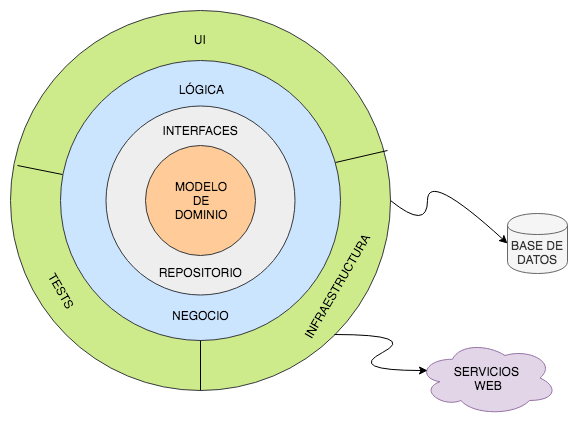
\includegraphics[width=15cm]{./chapters/img/architecture.png}

    \caption{Diagrama de la arquitectura}
    \label{fig:arch1}
\end{figure}

Además, se tiene una capa denominada Capa API, la cual consiste en una puerta de comunicación entre las peticiones de los usuarios y los servicios implementados. Esta capa está implementada utilizando el patrón de diseño \textit{Proxy}, se definen. Los usuarios no tendrán acceso directo a los servicios implementados, ni a la base de datos. La comunicación de la capa Interfaz de Usuario con los servicios solo es a través de la API.

Es importante destacar, que cada servicio que se representa en la Fig \ref{fig:arch1} incluye un representación de los datos que necesita de la base de datos. Esta representación se detalla en la Sección \ref{sec:data}, donde se indican los patrones de acceso a datos empleados. De esta forma se evita que de ser necesario algún cambio en algunas de las entidades de la base de datos, haya que re-implementar todos los servicios. En este caso, solo se afectan los servicios que utilizan estas entidades para su funcionamiento.